\documentclass[a4paper, 12pt, final, garamond]{book}
\usepackage{cours-preambule}

\makeatletter
\renewcommand{\@chapapp}{Devoir surveill\'e -- num\'ero}
\makeatother

\begin{document}
\setcounter{chapter}{4}

\chapter{Commentaires sur le DS n\degree05}

\section{Commentaires généraux}

Résultats très décevants, les commentaires du DS précédent sur la résonance
n'ont servi à rien. La mécanique, même rudimentaire, est mal traitée. Des
connaissances simples sur les ondes (propagation implique retard temporel) sont
gravement absentes. Moyenne à 09/20.

\begin{figure}[htbp!]
	\centering
	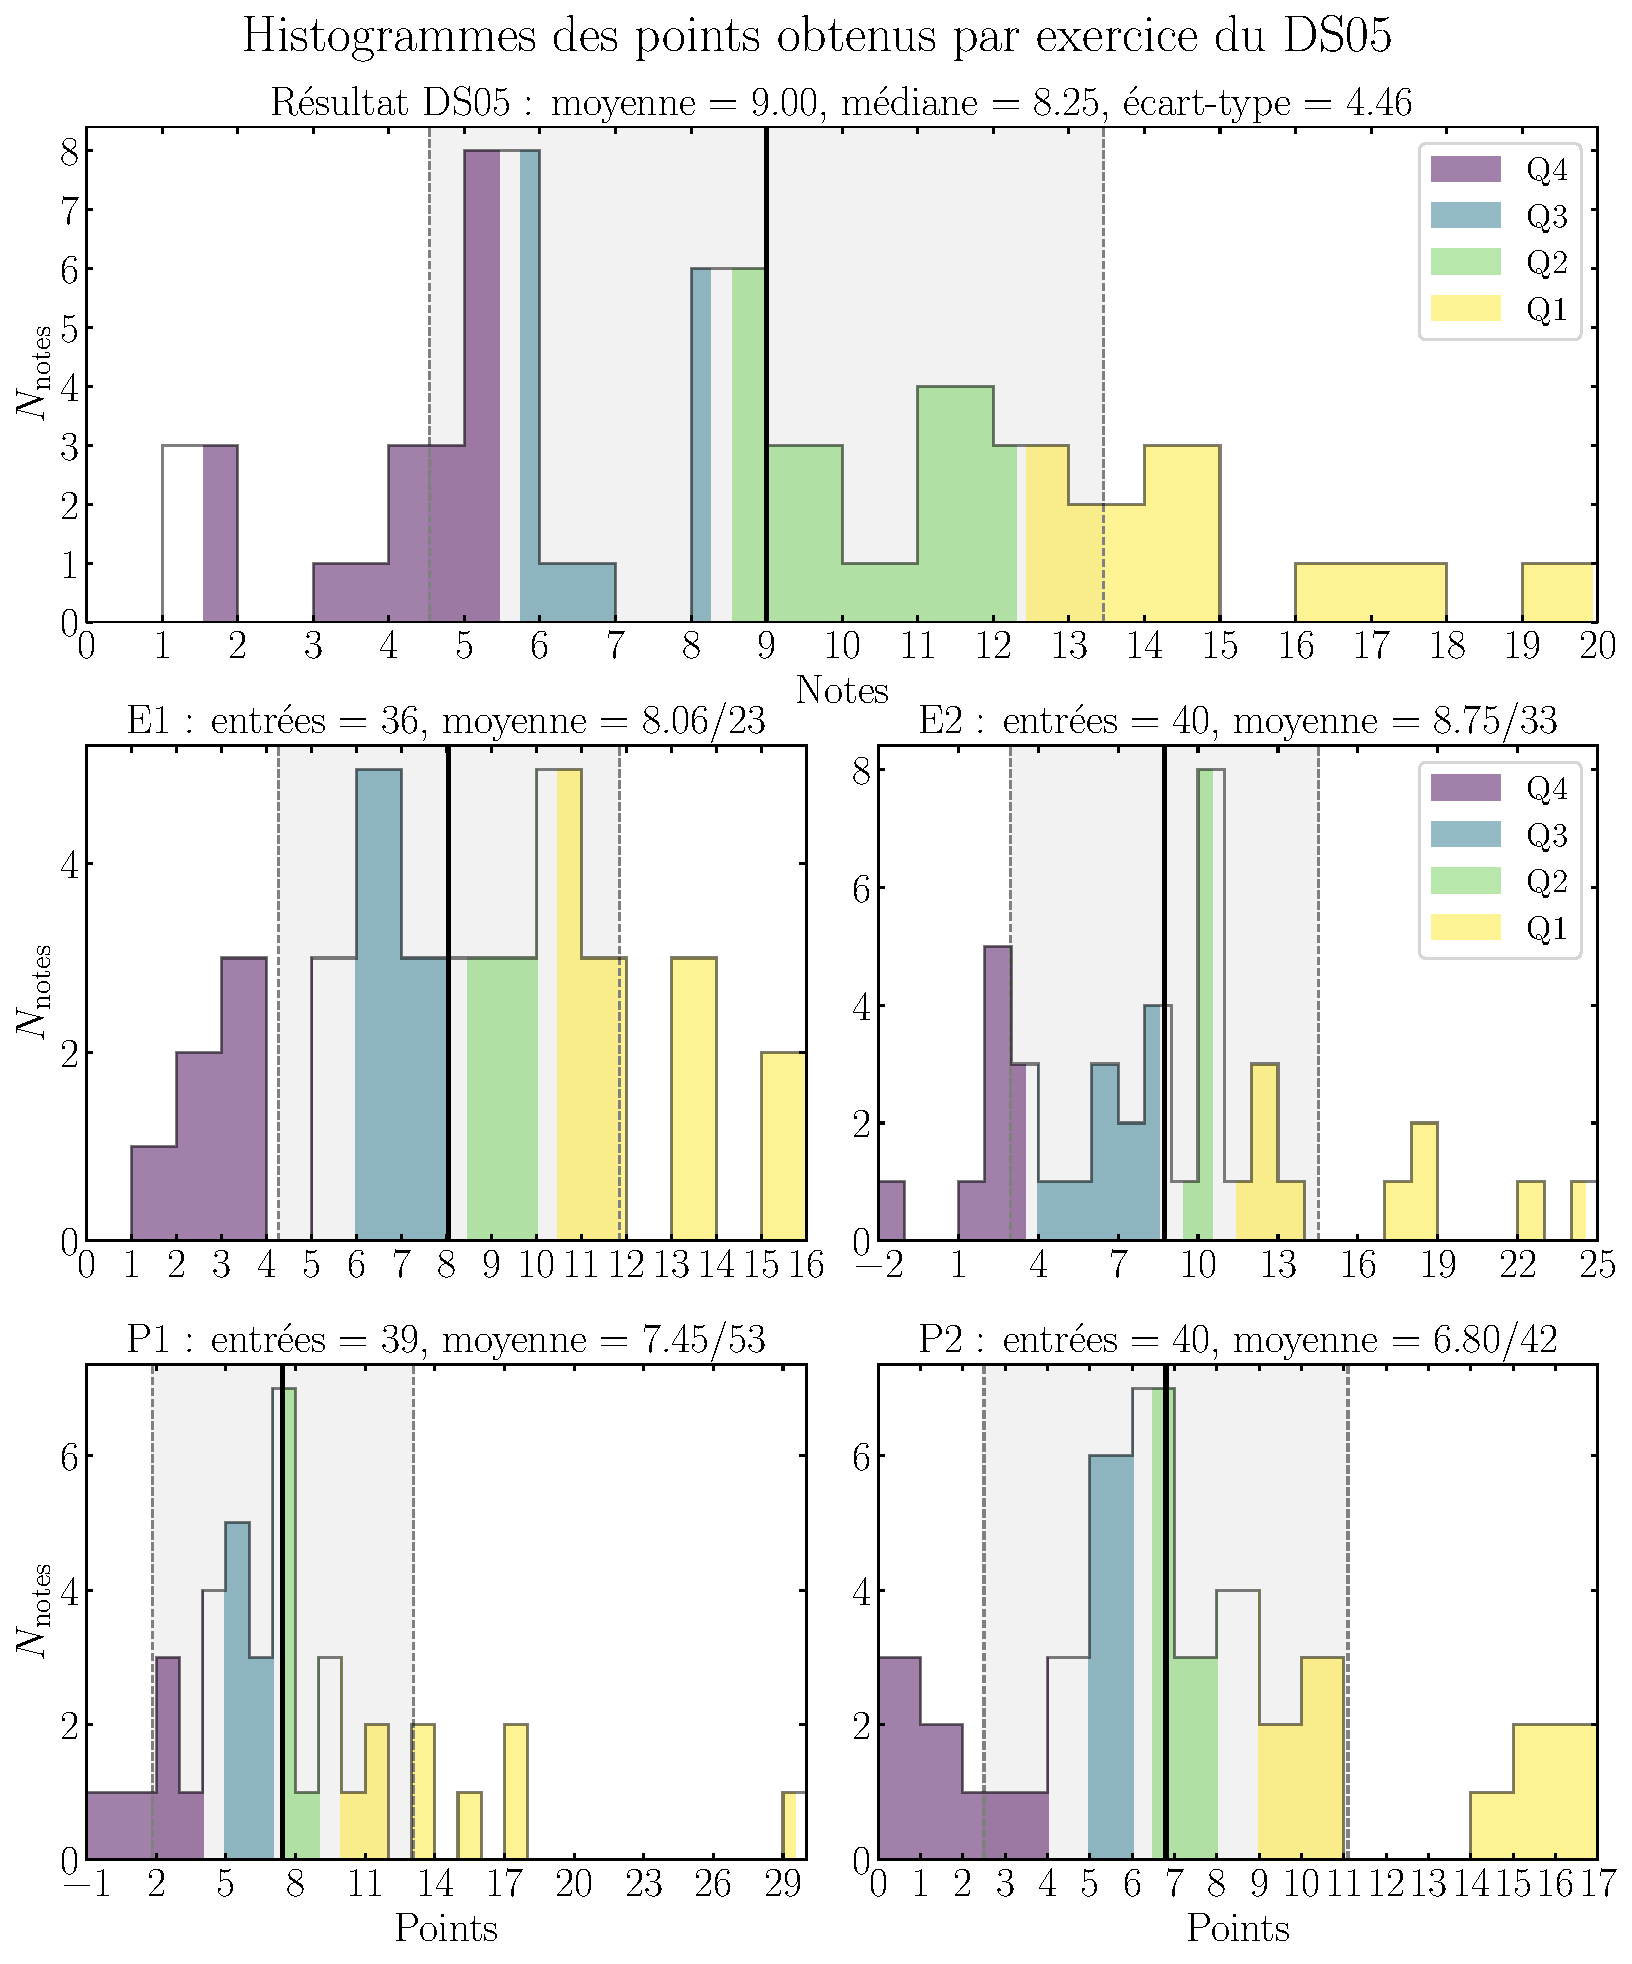
\includegraphics[width=.9\linewidth]{DS05_hist_all}
	\caption{Graphique des résultats}
\end{figure}

\setcounter{section}{0}
\exercice[22]{Ondes gravitationnelles}
\begin{enumerate}
	\nitem{6}% Q1
	Trop incomplet. Même nature et même fréquence avant toute chose, cohérence
	ensuite.
	\nitem{2}% Q2
	Correct.
	\nitem{5}% Q3
	Il fallait partir du retard temporel. \textbf{N'ajoutez pas des phases à
		l'origine} quand on vous a explicitement donné la forme du signal à l'origine,
	et ne négligez pas l'importance de ces chapitres sur les ondes. Ce sont des
	points faciles.
	\nitem{1}% Q4
	RAS.
	\nitem{1}% Q5
	RAS.
	\nitem{3}% Q6
	Correct.
	\nitem{3}% Q7
	Ne confondez pas le terme de phase à l'origine dans le signal sinusoïdal avec
	le déphasage dans l'amplitude du signal ! Erreur dans le corrigé, il faut
	$\ell_2- \ell_1 = \lambda/8$~: en effet, le terme dans le cos de l'amplitude
	est $\Delta\f_{1/2}/2$. Il faut revenir à la définition de $\Delta\f_{1/2} =
		-k\Delta{L_{1/2}}$~; on a bien $\Delta{L_{1/2}} = \fbox{2}(\ell_1 - \ell_2)$.
	\bigbreak
	\textbf{Ne pas travailler en congruences mais en ordre d'interférences}.
	\nitem{3}% Q8
	RAS.
\end{enumerate}

\exercice[33]{Chute d'une bille}
\begin{enumerate}
	\nitem{2}% Q1
	Poussée d'\textsc{Archimède} non connue. Aïe. Vous oubliez l'accélération de
	la pesanteur $\gf$~! Ça n'est pas normal d'oublier le volume d'une boule…
	\nitem{4}% Q2
	Réponses variées.
	\nitem{7}% Q3
	Globalement correct, mais vos schémas doivent faire apparaître les forces sur
	le système et le BDF doit être exprimé dans le repère choisi~! \textbf{Vous
		oubliez trop le repérage}.
	\nitem{3}% Q4
	Certain-es ont considéré que la bille avait changé de masse, et ont utilisé la
	masse volumique $\rho$ en facteur de $\af$ \textbf{et} en facteur de $\gf$… ça
	n'a aucun sens.
	\nitem{6}% Q5
	En fonction des données du problème, donc pas de $m$ qui n'est pas donné, mais
	du $4/3\,\pi R^{3}$~! Réponses avec $m$ acceptées.
	\smallbreak
	Des techniques d'adimensionnement random. J'avais insisté sur le fait qu'on vous
	le demande si nécessaire~: ne vous compliquez pas la vie pour rien~!
	\nitem{5}% Q6
	RAS.
	\nitem{1}% Q7
	Bien.
	\nitem{3}% Q8
	RAS.
	\nitem{2}% Q9
	Attention, \textbf{la viscosité n'est pas la masse volumique}. En effet, la
	glycérine est surtout plus visqueuse que l'eau ($\eta_g/\eta\ind{eau} \approx
		\num{1.45e3}$) et faiblement plus dense ($\rho_g/\rho\ind{eau} \approx
		\num{1.2}$). Ce qui permet à la bille d'atteindre sa vitesse limite c'est la
	viscosité.
\end{enumerate}

\setcounter{section}{0}
\prblm[53]{Microphone pour guitare}
\begin{enumerate}
	\nitem{6}% Q1
	Infiniment déçue des «~intensité nulle donc tension nulle~» pour un
	interrupteur ouvert… c'est accablant. Travaillez sincèrement les premières
	questions de régime permanent.
	\nitem{4}% Q2
	Il faut savoir faire le PdT dans le bon sens~!! C'est vraiment dommage d'avoir
	tant d'impédances équivalentes $Z\ind{eq} = 1/Z_{C_0} + 1/(Z_L+R_L)$~: c'est
	\textbf{clairement} inhomogène et \textbf{on ne fait pas d'impédance
		équivalente avec un générateur}~!! Faites les schémas représentant vos
	équivalences pour voir si c'est possible.
	\smallbreak
	$v = u_{C_0}$~: ils sont en parallèle~!
	\nitem{7}% Q3
	Soyez malin-es : $H_0$ ne dépend pas de $\w$. Il faut savoir identifier des
	expressions variables et constantes dans une équation. Ne vous précipitez pas
	pour dire $\w_0 = 1/\sqrt{LC_0}$ si ça n'est pas une évidence~: on identifie
	\textbf{après}~!
	\nitem{7}% Q4
	Vous n'avez pas retenu ce qu'est la résonance. Fâcheux. On voit ici la
	différence entre \textbf{comprendre} et \textbf{apprendre}~: si vous apprenez,
	alors vous oubliez au bout de 2 mois (résonance et associé vers novembre, DS
	en janvier). Si vous comprenez que pour trouver le maximum d'une fraction de
	numérateur constant, on cherche le minimum du dénominateur variable, tout se
	passe bien.
	\nitem{10}% Q5
	Souvent faux parce que c'était un passe-bas.
	\nitem{2}% Q6
	RAS.
	\nitem{2}% Q7
	RAS.
	\nitem{1}% Q8
	Il faut connaître ses définitions et vocabulaire…
	\nitem{5}% Q9
	RAS.
	\nitem{6}% Q10
	RAS.
	\nitem{3}% Q11
	RAS.
\end{enumerate}

\prblm[42]{Le bleu du ciel}
\begin{enumerate}
	\nitem{4}% Q1
	Dimensions $\neq $ unités ! $[F] = \si{N} = \si{kg.m.s^{-2}} \Lra \dim F =
		{\rm MLT^{-2}}$.
	\nitem{2}% Q2
	Bien.
	\nitem{4}% Q3
	TB.
	\nitem{2}% Q4
	$Q \gg 1 \dcancel{\Lra}$ régime transitoire long~: un grand facteur de qualité
	signifie qu'on aura \textbf{beaucoup d'oscillations}. Comme indiqué question
	5, $\tau = \frac{2Q}{\w_0}$, donc le régime transitoire dépend de $\w_0$.
	\nitem{9}% Q5
	Ici aussi, ne pas oublier les chapitres précédents et la résolution du régime
	pseudo-périodique d'un oscillateur amorti…
	\nitem{2}% Q6
	Définition du RSF.
	\nitem{4}% Q7
	Très peu traité.
	\nitem{3}% Q8
	RAS.
	\nitem{1}% Q9
	Il faut connaître les ordres de grandeurs extrêmes du visible~: $\lambda \in
		\SIrange{400}{800}{nm}$.
	\nitem{2}% Q10
	$\w = 2\pi f$. Faites attention à l'homogénéité.
	\nitem{1}% Q11
	RAS.
	\nitem{2}% Q12
	Pas traitée.
	\nitem{2}% Q13
	C'était honnêtement traitable juste en lisant l'énoncé~: vous aviez $X_m$ dans
	la question précédente.
	\nitem{2}% Q14
	Dommage.
	\nitem{2}% Q15
	Quelques explications assez fantastiques.
\end{enumerate}

\end{document}
